% -*- TeX-engine: luatex -*-
\documentclass[presentation,aspectratio=43, 10pt]{beamer}
\usepackage{pifont}
\newcommand{\cmark}{\ding{51}}
\newcommand{\xmark}{\ding{55}}

\usepackage{booktabs}
\titlegraphic{\hfill
\includegraphics[height=1.25cm]{durham-logo}}
\usepackage{appendixnumberbeamer}
\usepackage{amsmath}
\usepackage{amssymb}
\usepackage{mathtools}
\usepackage{hyperref}
\usepackage{xspace}
\newcommand{\arxivlink}[2]{{\texttt{arXiv:\,\href{https://arxiv.org/abs/#1}{#1\,[#2]}}}}

\newcommand{\honev}{\ensuremath{{H}^1(\Omega; \mathbb{R}^d)}\xspace}
\newcommand{\ltwov}{\ensuremath{{L}^2(\Omega; \mathbb{R}^d)}\xspace}
\newcommand{\ltwo}{\ensuremath{{L}^2(\Omega)}\xspace}
\newcommand{\inner}[1]{\left\langle #1 \right \rangle}
\newcommand{\dx}{\,\text{d}x}
\newcommand{\ds}{\,\text{d}s}


\usepackage{minted}
\usepackage[url=false,
doi=true,
isbn=false,
style=authoryear,
maxnames=5,
giveninits=true,
uniquename=init,
backend=biber]{biblatex}
\renewcommand{\bibfont}{\fontsize{7}{7}\selectfont}
\addbibresource{../literature.bib}

\setlength{\bibitemsep}{1ex}
\setlength{\fboxsep}{1pt}

\renewbibmacro{in:}{}
\DeclareFieldFormat[article]{volume}{\textbf{#1}}
\DeclareFieldFormat{doi}{%
  doi\addcolon%
  {\scriptsize\ifhyperref{\href{http://dx.doi.org/#1}{\nolinkurl{#1}}}
    {\nolinkurl{#1}}}}
\AtEveryBibitem{%
\clearfield{pages}%
\clearfield{issue}%
\clearfield{number}%
}

\DeclareMathOperator{\grad}{grad}
\let\div\relax
\DeclareMathOperator{\div}{div}
\DeclareMathOperator{\curl}{curl}
\DeclareMathOperator{\range}{range}
\DeclareMathOperator{\sym}{sym}
\usetheme{metropolis}
\setbeamertemplate{title graphic}{
  \vbox to 0pt {
    \vspace*{1em}
    \inserttitlegraphic%
  }%
  \nointerlineskip%
}
\metroset{background=light,progressbar=frametitle,numbering=counter,block=fill}

% https://www.dur.ac.uk/marketingandcommunications/marketing/branding/colourpalette/
% Most of these are indistinguishable to those suffering colour blindness
\definecolor{purple}{HTML}{68246D}
\definecolor{blue}{HTML}{002A41}
\definecolor{red}{HTML}{BE1E2D}
\definecolor{cyan}{HTML}{00AEEF}
\definecolor{yellow}{HTML}{FFD53A}

\newenvironment{variableblock}[3]
{\setbeamercolor{block body}{#2}
\setbeamercolor{block title}{#3}
\begin{block}{#1}}%
{\end{block}}
  
\newenvironment{challenge}[1]%
{\begin{variableblock}{#1}{bg=red!20,fg=black}{bg=red,fg=white}}%
{\end{variableblock}}

\newenvironment{answer}[1]%
{\begin{variableblock}{#1}{bg=cyan!20,fg=black}{bg=cyan,fg=white}}%
{\end{variableblock}}

\renewenvironment{exampleblock}[1]%
{\begin{variableblock}{#1}{bg=yellow!20,fg=black}{bg=yellow,fg=white}}%
{\end{variableblock}}

\setbeamercolor{normal text}{
  fg=black,
  bg=white
}
\setbeamercolor{alerted text}{
  fg=red
}
\setbeamercolor{example text}{
  fg=blue
}

\setbeamercolor{palette primary}{%
  use=normal text,
  fg=normal text.bg,
  bg=purple,
}

\usetheme{metropolis}

\author{Lawrence Mitchell\inst{1,*}}
\institute{
  \inst{1}Department of Computer Science, Durham University\\
  \inst{*}\texttt{lawrence.mitchell@durham.ac.uk}}

\title{Flexible computational abstractions in the design and
  implementation of multiphysics preconditioners}

\usepackage{tikz}
\usetikzlibrary{trees,calc,positioning}
\usetikzlibrary{shapes, shapes.geometric}
\usetikzlibrary{arrows,chains,positioning,fit,backgrounds,calc,shapes,
  shadows,scopes,decorations.markings,plotmarks}

\newcommand*{\tettextsize}{\footnotesize}
\tikzstyle{line} = [draw, -, thick]
\tikzstyle{nodraw} = [draw, fill, circle, minimum width=0pt, inner sep=0pt]
\tikzstyle{sieve} = [line, circle, font=\tettextsize, inner sep=0pt,
  minimum size=12pt]

\tikzstyle{cell} = [sieve, fill=blue!60]
\tikzstyle{facet} = [sieve, fill=green!35]
\tikzstyle{edge} = [sieve, fill=red!35]
\tikzstyle{vertex} = [sieve, fill=blue!35]

% https://tex.stackexchange.com/questions/27171/padded-boundary-of-convex-hull
\newcommand{\convexpath}[2]{
  [
  create hullcoords/.code={
    \global\edef\namelist{#1}
    \foreach [count=\counter] \nodename in \namelist {
      \global\edef\numberofnodes{\counter}
      \coordinate (hullcoord\counter) at (\nodename);
    }
    \coordinate (hullcoord0) at (hullcoord\numberofnodes);
    \pgfmathtruncatemacro\lastnumber{\numberofnodes+1}
    \coordinate (hullcoord\lastnumber) at (hullcoord1);
  },
  create hullcoords
  ]
  ($(hullcoord1)!#2!-90:(hullcoord0)$)
  \foreach [
  evaluate=\currentnode as \previousnode using \currentnode-1,
  evaluate=\currentnode as \nextnode using \currentnode+1
  ] \currentnode in {1,...,\numberofnodes} {
    let \p1 = ($(hullcoord\currentnode) - (hullcoord\previousnode)$),
    \n1 = {atan2(\y1,\x1) + 90},
    \p2 = ($(hullcoord\nextnode) - (hullcoord\currentnode)$),
    \n2 = {atan2(\y2,\x2) + 90},
    \n{delta} = {Mod(\n2-\n1,360) - 360}
    in
    {arc [start angle=\n1, delta angle=\n{delta}, radius=#2]}
    -- ($(hullcoord\nextnode)!#2!-90:(hullcoord\currentnode)$)
  }
}

\graphicspath{{./\jobname.figures/}{../pictures/}}

\begin{document}
\maketitle

% \begin{abstract}
%   Small block overlapping, and non-overlapping, Schwarz methods are
%   theoretically highly attractive as multigrid smoothers for a wide
%   variety of problems that are not amenable to point relaxation
%   methods. Examples include monolithic Vanka smoothers for Stokes,
%   overlapping vertex-patch decompositions for $H(\text{div})$ and
%   $H(\text{curl})$ problems, and line smoothers for elliptic problems
%   in thin domains.

%   While it is possible to manually program these different schemes,
%   their use in general purpose libraries has been held back by a lack
%   of generic, composable interfaces. I present a new approach to the
%   specification and development such additive Schwarz methods in PETSc
%   that cleanly separates the topological space decomposition from the
%   discretisation and assembly of the equations. This separation
%   enables both linear and nonlinear smoothers to be supported through
%   the same callback interface.

%   The preconditioner is flexible enough to support overlapping and
%   non-overlapping additive Schwarz methods, and can be used to
%   formulate line, and plane smoothers, Vanka iterations, and others. I
%   will illustrate the effectiveness with examples using the Firedrake
%   finite element library.
% \end{abstract}

\begin{frame}[t]
  \frametitle{Setting}

  \begin{columns}
    \begin{column}{0.8\textwidth}
      \begin{quote}
        Firedrake \url{www.firedrakeproject.org} {\normalfont
          [\ldots]} is an automated system for the solution of
        partial differential equations using the finite element
        method.
      \end{quote}
    \end{column}
    \begin{column}{0.2\textwidth}
      
\includegraphics[width=0.8\textwidth]{firedrake}
    \end{column}
  \end{columns}
  \begin{itemize}
  \item Uses \emph{embedded} domain specific language, UFL
    \parencite{Alnaes:2014} from the FEniCS project.
  \item PETSc for meshes and (algebraic) solvers.
  \item \alert{Flexible preconditioning framework for problem-specific
    multigrid and block preconditioning}
  \end{itemize}

  {\raggedleft
    \scriptsize \textcite{Rathgeber:2016} \arxivlink{1501.01809}{cs.MS}\par}
\end{frame}

\begin{frame}[fragile, t]
  \frametitle{Discretisation becomes ``easy''}
  \begin{columns}[T]
    \begin{column}{0.47\framewidth}
      \begin{block}{Rayleigh-B\'enard convection}      
        \footnotesize
        Find $(u, p, T) \in V\times W\times Q$ s.t.
        \begin{align*}
          \int_\Omega\nabla u : \nabla v + \int_\Omega (u \cdot \nabla u) \cdot v \\
          - \int_\Omega p \nabla\cdot v + \frac{\text{Ra}}{\text{Pr}}
          \int_\Omega Tg\hat{z} \cdot v &= 0 \\
          \int_\Omega \nabla\cdot u q &= 0\\
          \int_\Omega \nabla T \cdot u S
          + \text{Pr}^{-1} \int_\Omega \nabla T \cdot \nabla S &= 0\\
          \quad \text{for all } (v,q,S) \in V\times W \times Q
        \end{align*}      
        Newton
        \begin{equation*}
          \begin{bmatrix}
            F   & B^T & M_1 \\
            C   & 0   & 0   \\
            M_2 & 0 & K
          \end{bmatrix}
          \begin{bmatrix}
            \delta u \\
            \delta p \\
            \delta T
          \end{bmatrix} =
          \begin{bmatrix}
            f_1 \\
            f_2 \\
            f_3
          \end{bmatrix}
        \end{equation*}
      \end{block}
    \end{column}
    \begin{column}{0.52\framewidth}
\begin{minted}[fontsize=\tiny]{python}
from firedrake import *
mesh = Mesh(...)
V = VectorFunctionSpace(mesh, "CG", 2)
W = FunctionSpace(mesh, "CG", 1)
Q = FunctionSpace(mesh, "CG", 1)
Z = V * W * Q
Ra = Constant(200)
Pr = Constant(6.18)
upT = Function(Z)
u, p, T = split(upT)
v, q, S = TestFunctions(Z)
bcs = [...] # no-flow + temp gradient
nullspace = MixedVectorSpaceBasis(
   Z, [Z.sub(0), VectorSpaceBasis(constant=True),
       Z.sub(2)])
F = (inner(grad(u), grad(v))
     + inner(dot(u, grad(u)), v)
     - inner(p, div(v))
     + (Ra/Pr)*inner(T*g, v)
     + inner(div(u), q)
     + inner(dot(grad(T), u), S)
     + (1/Pr) * inner(grad(T), grad(S)))*dx

solve(F == 0, upT, bcs=bcs, nullspace=nullspace)
\end{minted}
    \end{column}
  \end{columns}
\end{frame}


\begin{frame}[t]
  \frametitle{Now we can get stuck on the solver\dots}
  \begin{onlyenv}<1>
    \begin{block}{Stokes equations}
      \begin{alignat*}{2}
        -\nabla^2 u + \nabla p &= f \quad && \text{ in } \Omega, \\
        \nabla \cdot u &= 0 \quad && \text{ in } \Omega, \\
      \end{alignat*}

      Discretising with inf-sup stable element pair results in:
      \begin{equation*}
        Jx := \begin{bmatrix}
          A & B^T \\
          B & 0
        \end{bmatrix}
        \begin{bmatrix}
          u \\ p
        \end{bmatrix}
        =
        \begin{bmatrix}
          b \\ 0
        \end{bmatrix}.
      \end{equation*}
    \end{block}
  \end{onlyenv}
  \begin{onlyenv}<2>
    \begin{block}{\dots and a preconditioner}
      Use a diagonal Schur complement factorisation
      \parencite{Silvester:1994}
      \begin{equation*}
        \tilde{J}^{-1} =
        \begin{bmatrix}
          \tilde{A}^{-1}  & 0 \\
          0 & \tilde{S}^{-1} \\
        \end{bmatrix}
      \end{equation*}

      With multigrid for $\tilde{A}^{-1}$, and
      $\tilde{S}^{-1} = -Q^{-1}$ ($Q$ the pressure mass matrix).
    \end{block}
  \end{onlyenv}
  \begin{onlyenv}<3>
    \begin{block}{Stationary Rayleigh-B\'enard convection}
      \begin{equation*}
        \begin{split}
          -\Delta u + u\cdot\nabla u + \nabla p +
          \frac{\text{Ra}}{\text{Pr}} \hat{g}T &= 0 \\
          \nabla \cdot u &= 0 \\
          - \frac{1}{\text{Pr}} \Delta T + u\cdot \nabla T &= 0
        \end{split}
      \end{equation*}
      Newton linearisation
      \begin{equation*}
        \begin{bmatrix}
          F   & B^T & M_1 \\
          C   & 0   & 0   \\
          M_2 & 0 & K
        \end{bmatrix}
        \begin{bmatrix}
          \delta u \\
          \delta p \\
          \delta T
        \end{bmatrix} =
        \begin{bmatrix}
          f_1 \\
          f_2 \\
          f_3
        \end{bmatrix}
      \end{equation*}
    \end{block}
  \end{onlyenv}
  \begin{onlyenv}<4>
    \begin{block}{\dots and a preconditioner}
      {\small For each Newton step, invert the $3\times 3$ block
        system using a preconditioner from \textcite{Howle:2012}:
        \begin{equation*}
          \begin{bmatrix}
            \widetilde{\begin{bmatrix}
                F & B^T\\
                C & 0
              \end{bmatrix}}^{-1} & 0\\
            0 & I
          \end{bmatrix}
          \begin{bmatrix}
            I & 0 & -M_1\\
            0 & I & 0 \\
            0 & 0 & I
          \end{bmatrix}
          \begin{bmatrix}
            I & 0 & 0\\
            0 & I & 0\\
            0 & 0 & \tilde{K}^{-1}
          \end{bmatrix}
        \end{equation*}
        with
        \begin{equation*}
          \widetilde{\begin{bmatrix}
              F & B^T\\
              C & 0
            \end{bmatrix}}^{-1} = \begin{bmatrix}
            F & 0 \\
            0 & \tilde{S}^{-1}
          \end{bmatrix}
          \begin{bmatrix}
            I & 0\\
            -C & I
          \end{bmatrix}
          \begin{bmatrix}
            \tilde{F}^{-1} & 0 \\
            0 & I
          \end{bmatrix}
        \end{equation*}
        with $S = -C \tilde{F}^{-1} B^T$ the Schur complement, whose
        inverse is approximated with PCD:
        \begin{equation*}
          \tilde{S}^{-1} = \tilde{M}_p^{-1}(\mathbb{I} + F_p \tilde{L}_p^{-1})
        \end{equation*}
      }
    \end{block}
  \end{onlyenv}
  \begin{onlyenv}<5>
    \begin{block}{Time dependent Stokes}
      Implicit time-stepping schemes lead to a saddle-point system
      \begin{equation*}
        \begin{bmatrix}
          I - \epsilon^2 \Delta & -\grad\\
          \div & 0
        \end{bmatrix}.
      \end{equation*}
      For which the ``canonical'' diagonal block preconditioner is
      \begin{equation*}
        \begin{bmatrix}
          (I - \epsilon^2 \Delta)^{-1} & 0\\
          0 & (-\Delta)^{-1} + \epsilon^2 I
        \end{bmatrix}.
      \end{equation*}
      \begin{flushright}
        \textcite{Mardal:2011} \hspace{4em}
      \end{flushright}
    \end{block}
  \end{onlyenv}

\end{frame}

\begin{frame}
  \frametitle{Unifying observation}
  \begin{block}{Auxiliary operators}
    Many schemes require access, \emph{in the preconditioner}, to
    matrix blocks that are not in the original operator.
  \end{block}
  \begin{example}
    \begin{itemize}
    \item PCD requires a pressure Laplacian, mass matrix, and
      convection
    \item Time dependent Stokes needs a pressure Laplacian, and mass
      matrix
    \end{itemize}
  \end{example}
  \begin{itemize}
  \item These operators are typically \emph{easy} for the
    discretisation library to build.
  \item How do we get them into the solver?
  \end{itemize}
\end{frame}

\begin{frame}
  \frametitle{Composition}

  Follow PETSc philosophy of runtime composition
  \begin{block}{Idea}
    \begin{itemize}
    \item Endow discretised operators with PDE-level information:
      \begin{itemize}
      \item what equation/function space?
      \item boundary conditions, etc\ldots
      \end{itemize}
    \item Enable use of PETSc's \texttt{fieldsplit} preconditioner for
      these operators
    \item[$\Rightarrow$] gets access to all the block factorisation
      schemes
    \item[\cmark] PETSc provides \emph{algebraic} composition of solvers. \nocite{Brown:2012}
    \item[\cmark] Firedrake can provide auxiliary operators
    \item[\xmark?] Require model developer to write a preconditioner
    \end{itemize}
  \end{block}
  {\raggedleft \scriptsize
    \textcite{Kirby:2018} \arxivlink{1706.01346}{cs.MS}\par}
\end{frame}
\begin{frame}[fragile]
  \frametitle{Example: that Stokes PC}
\begin{minted}[fontsize=\scriptsize]{python}
from firedrake import *                  # Params set up as
...                                      -ksp_type gmres
V = VectorFunctionSpace(mesh, "CG", 2)   -pc_type fieldsplit
Q = FunctionSpace(mesh, "CG", 1)         -pc_fieldsplit_type schur
W = V*Q                                  -pc_fieldsplit_schur_fact_type diag
v, q = TestFunctions(W)                  -fieldsplit_0_
                                            -ksp_type preonly
w = Function(W)                             -pc_type gamg
u, p = split(w)                          -fieldsplit_1_
F = (inner(grad(u), grad(v))*dx             -ksp_type chebyshev
    - p*div(v)*dx - div(u)*q*dx             -ksp_max_it 2
                                            -pc_type python
                                            # Callback to Firedrake
class MassMatrix(AuxiliaryOperatorPC):      -pc_python_type MassMatrix
    _prefix = "mass_"                       -mass_pc_type sor
    def form(self, pc, test, trial):
        a = -inner(test, trial)*dx
        return (a, None)

solve(F == 0, w, solver_parameters=params)
\end{minted}
\end{frame}

\begin{frame}
  \frametitle{What about those Schur complements?}
  \begin{columns}
    \begin{column}{0.55\textwidth}
      Want an approximation $\tilde{S}^{-1}$ that
      \begin{enumerate}
      \item is robust to parameter variation
      \item is cheap to construct/apply
      \item scales well in parallel
      \end{enumerate}

      Generally (1) is the hardest to satisfy.

      $\Rightarrow$ augmented Lagrangian approach.
    \end{column}
    \begin{column}{0.45\textwidth}
      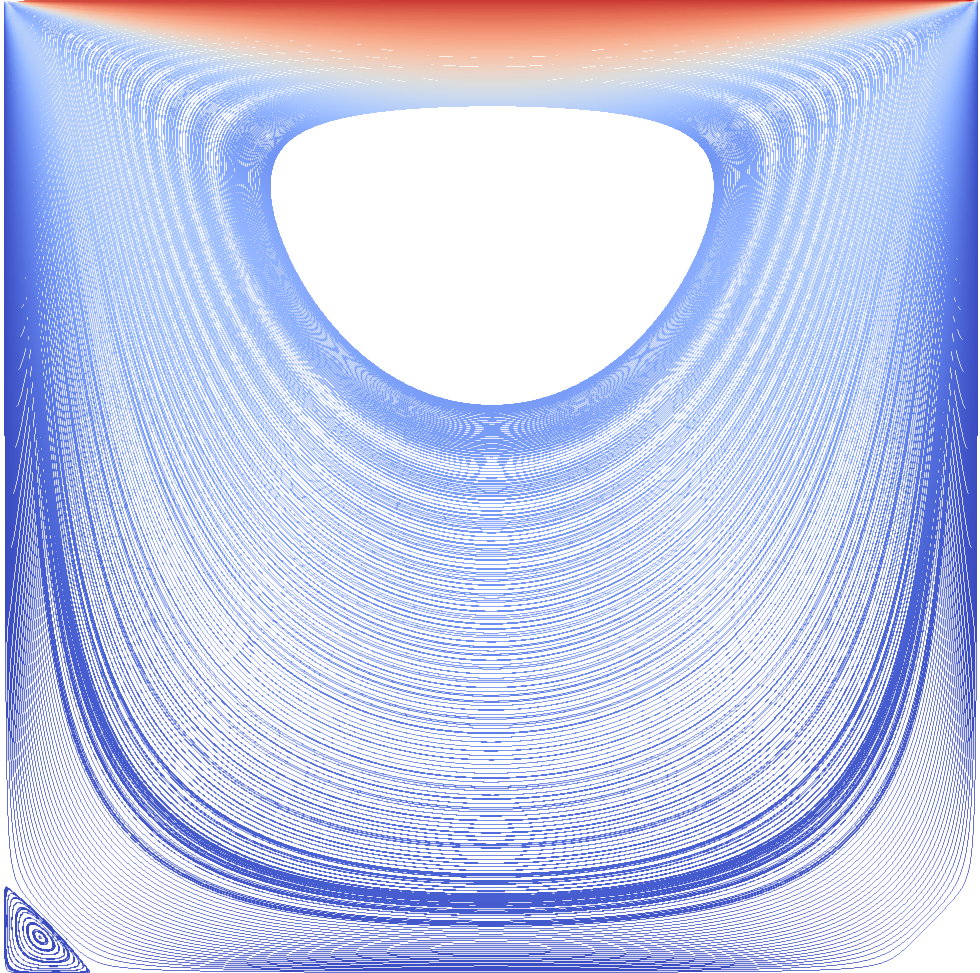
\includegraphics[width=0.333\textwidth]{mhd/ldc_1_1_u}%
      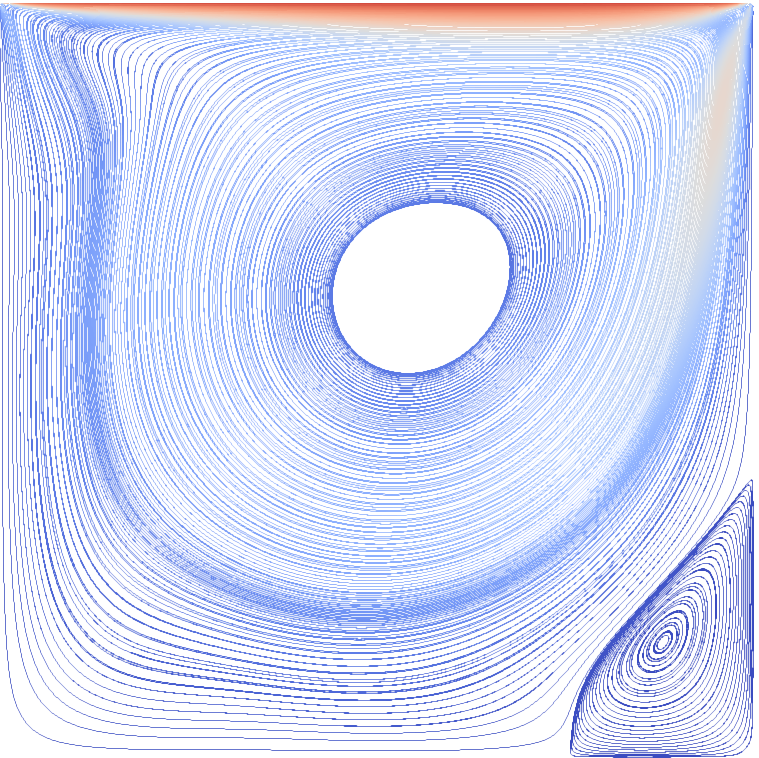
\includegraphics[width=0.333\textwidth]{mhd/ldc_500_500_u}%
      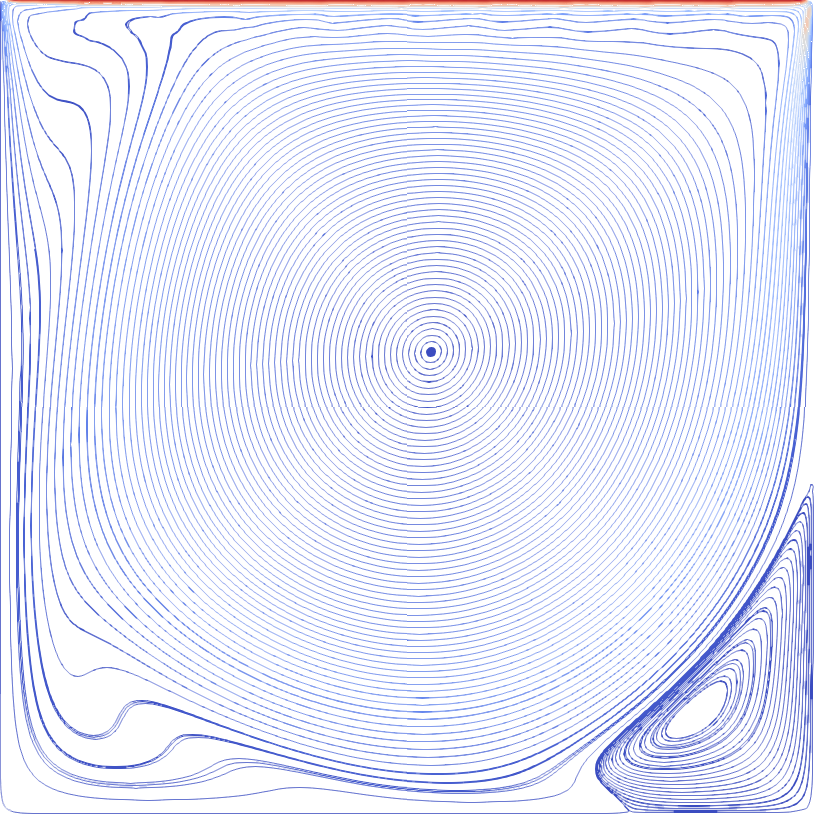
\includegraphics[width=0.333\textwidth]{mhd/ldc_5000_5000_u}%
      \\
      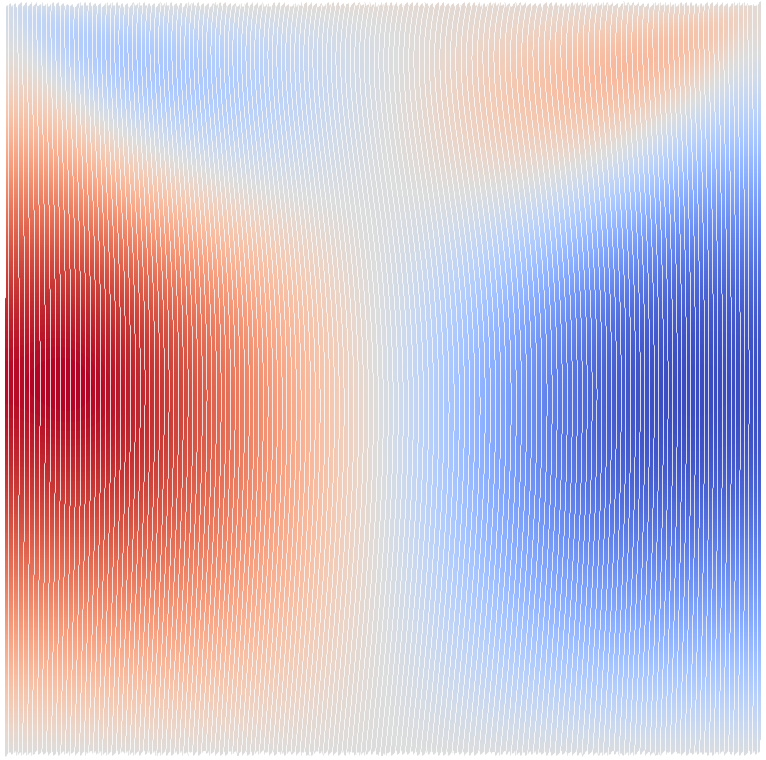
\includegraphics[width=0.333\textwidth]{mhd/ldc_1_1_B}%
      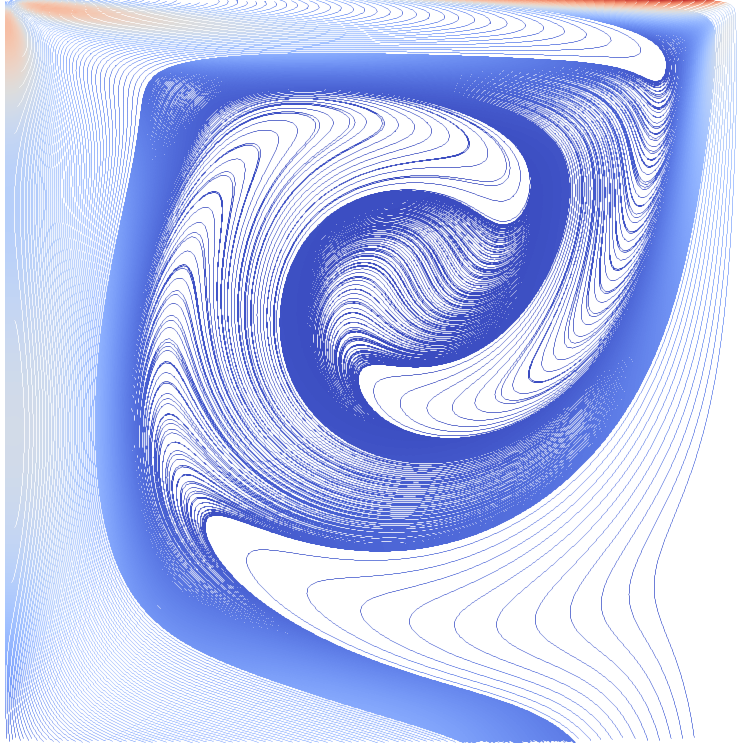
\includegraphics[width=0.333\textwidth]{mhd/ldc_500_500_B}%
      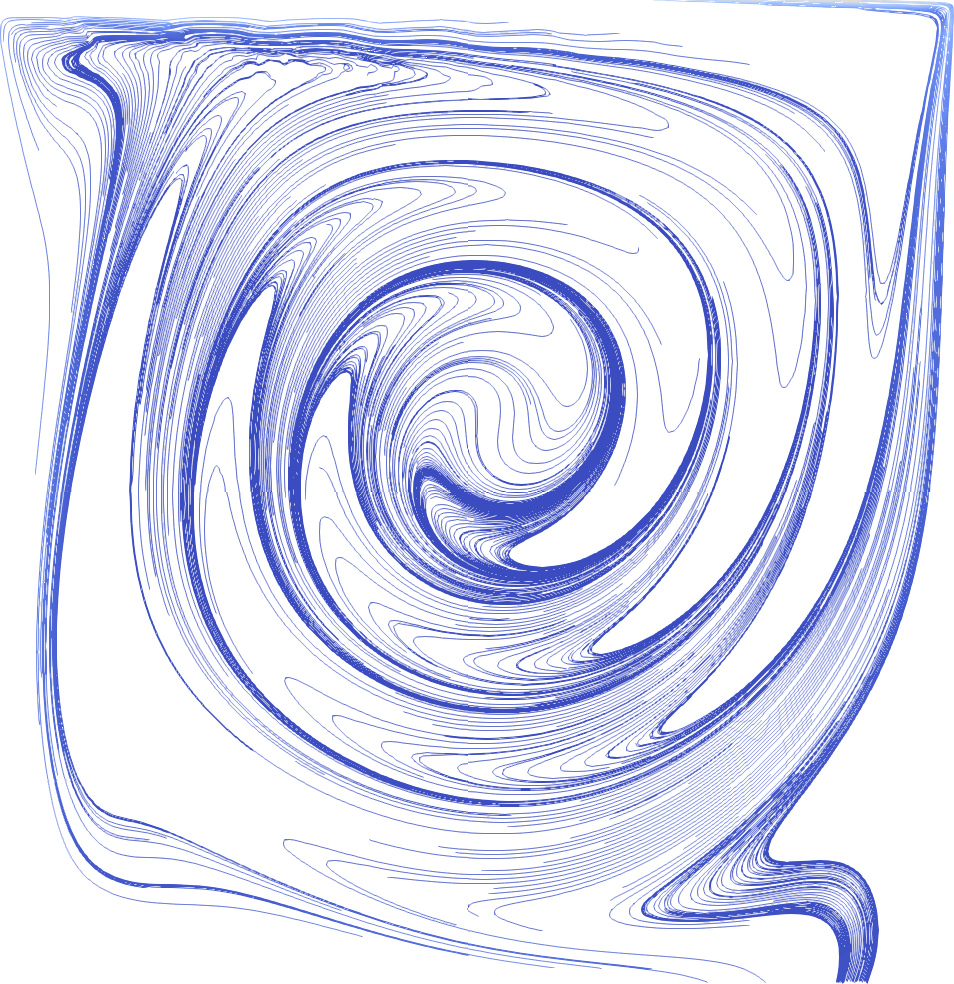
\includegraphics[width=0.333\textwidth]{mhd/ldc_5000_5000_B}%

      \vspace{2em}
      {\raggedleft\scriptsize
        \textcite{Laakmann:2021} \arxivlink{2104.14855}{math.NA}\par}
    \end{column}
  \end{columns}
\end{frame}

\begin{frame}
  \frametitle{Augmented Lagrangian methods}
  \begin{itemize}
  \item Originally a way of stabilising finite element methods for
    elasticity and fluids \parencite{Fortin:1983}
  \item More recently, part of a preconditioning strategy for coupled
    problems with a constraint
    \parencite{Benzi:2006,Farrell:2019,Farrell:2021a,Shih:2021}, \dots
  \end{itemize}
  \begin{block}{Idea}
    Add a penalisation of the constraint to the momentum equation

    \begin{equation*}
      (u \cdot \nabla) u + \nabla p \alert{- \gamma \nabla \nabla
        \cdot u} - \nu \nabla^2 u = 0, \quad\quad \nabla \cdot u = 0
    \end{equation*}
  \end{block}
\end{frame}

\begin{frame}
  \frametitle{Why? Schur complement approximation is \emph{easy!}}
  Example: for Navier--Stokes, after discretisation and linearisation,
  Jacobian is now
  \begin{equation*}
    \begin{pmatrix}
      A + \gamma B^T M_p^{-1} B & B^T \\
      B & 0
    \end{pmatrix}
    \begin{pmatrix}
      u \\ p
    \end{pmatrix}
    =
    \begin{pmatrix}
      b \\ 0
    \end{pmatrix}
  \end{equation*}

  \begin{answer}{Good news!}
    As $\gamma \to \infty$, $S^{-1}$ is well approximated by
    $\tilde{S}^{-1} = -(\nu + \gamma)M_p^{-1}$.
  \end{answer}
  \pause
  \begin{challenge}{Bad news!}
    $A_\gamma \coloneqq A + \gamma B^T M_p^{-1} B$ is \emph{much}
    harder to invert than $A$.
  \end{challenge}
\end{frame}

\begin{frame}
  \frametitle{More solver technology: \texttt{PCPATCH}}
  (Small-block) overlapping Schwarz smoothers
  \begin{itemize}
  \item Separate topological decomposition from algebraic operators
  \item Ask discretisation library to make the operators once
    decomposition is obtained
  \end{itemize}
  \begin{block}{Topological decomposition}
    Use \texttt{DMPlex} to provide decomposition of mesh into patches.
  \end{block}

  \begin{block}{Space decomposition}
    Use topological decomposition plus \texttt{PetscSection} to
    determine degrees of freedom in each patch.
  \end{block}

  \begin{block}{Operators}
    Callback interface to discretisation/PDE library.
  \end{block}

  {\raggedleft
    \scriptsize \textcite{Farrell:2021b} \arxivlink{1912.08516}{cs.MS}\par}
\end{frame}

\begin{frame}[fragile]
 \frametitle{Topological subspace definition via \texttt{DMPlex}}
 \begin{itemize}
 \item Each patch defined by set of mesh points (entities) on which the dofs
   we're going to solve for in the patch live
 \end{itemize}
 \begin{block}{Builtin}
   Specify patches by selecting:
   \begin{enumerate}
   \item Mesh points $\{p_i\}$ to iterate over (e.g.~vertices, cells)
   \item Adjacency relation that gathers points in patch
     \begin{itemize}
     \item[\texttt{star}] points in $\text{star}(p_i)$
     \item[\texttt{vanka}] points in
       $\text{closure}(\text{star}(p_i))$
     \item[\texttt{pardecomp}] process-local part of mesh (for
       nonlinear DD).
     \end{itemize}
   \end{enumerate}
 \end{block}
 \begin{block}{User-defined}
   Callback provides list of entities in each patch, plus iteration order.
 \end{block}
\end{frame}

\begin{frame}
  \frametitle{What subspace to choose?}
  \begin{onlyenv}<1> Consider the problem: for
    $\alpha, \beta \in \mathbb{R}$, find $u \in V$ such that
    \begin{equation*}
      \alpha a(u, v) + \beta b(u, v) = (f, v) \quad \forall v \in V,
    \end{equation*}
    where $a$ is SPD, and $b$ is symmetric positive semidefinite.
  \end{onlyenv}
  \begin{theorem}[Sch\"oberl (1999); Lee, Wu, Xu, Zikatanov (2007)]
    \small
    Let the kernel be
    \begin{equation*}
      \mathcal{N} := \{ u \in V : b(u, v) = 0 \,\, \forall v \in V \}.
    \end{equation*}
    If the subspace decomposition \emph{captures the kernel}
    \begin{equation*}
      \mathcal{N} = \sum_i \mathcal{N} \cap V_i,
    \end{equation*}
    then convergence of the relaxation defined by this decomposition
    will be \emph{independent} of $\alpha$ and $\beta$.
    \nocite{Schoeberl:1999,Lee:2007}
  \end{theorem}
  \begin{onlyenv}<2>
    \begin{corollary}
      \small
      ``All'' we need to do is characterise the kernel: in particular
      the support of the basis.

      Appropriate discrete de Rham complexes can help.
    \end{corollary}
  \end{onlyenv}
\end{frame}

\begin{frame}[fragile,t]
  \frametitle{Divergence free Navier--Stokes with augmented Lagrangian}
  \vspace{-1.5\baselineskip}
  {\small\begin{equation*}
    \text{Find $u \in (H^1)^d$ s.t.}\quad \nu(\grad u, \grad v) + (u\cdot \grad u, v) + \gamma(\div u, \div v) = (f, v) \quad \forall v \in V.
  \end{equation*}}
  \vspace*{-\baselineskip}
  \begin{block}{Stokes complex on Alfeld splits}
    \begin{equation*}
      \mathbb{R} \xrightarrow{\operatorname{id}} H^2 \xrightarrow{\grad} H^1(\curl)
      \xrightarrow{\curl} H^1 \xrightarrow{\div} L^2 \xrightarrow{\operatorname{null}} 0,
    \end{equation*}
    Decomposition must capture $\ker \div = \range \curl$.

    Appropriate discrete spaces are constructed in \textcite{Fu:2018}: use
    barycentrically refined meshes, piecewise continuous space with $k
    \ge d$, ``macro star'' patch around vertices.
  \end{block}
  \begin{overlayarea}{\textwidth}{0.4\textheight}
    \begin{onlyenv}<1>
      \begin{center}
        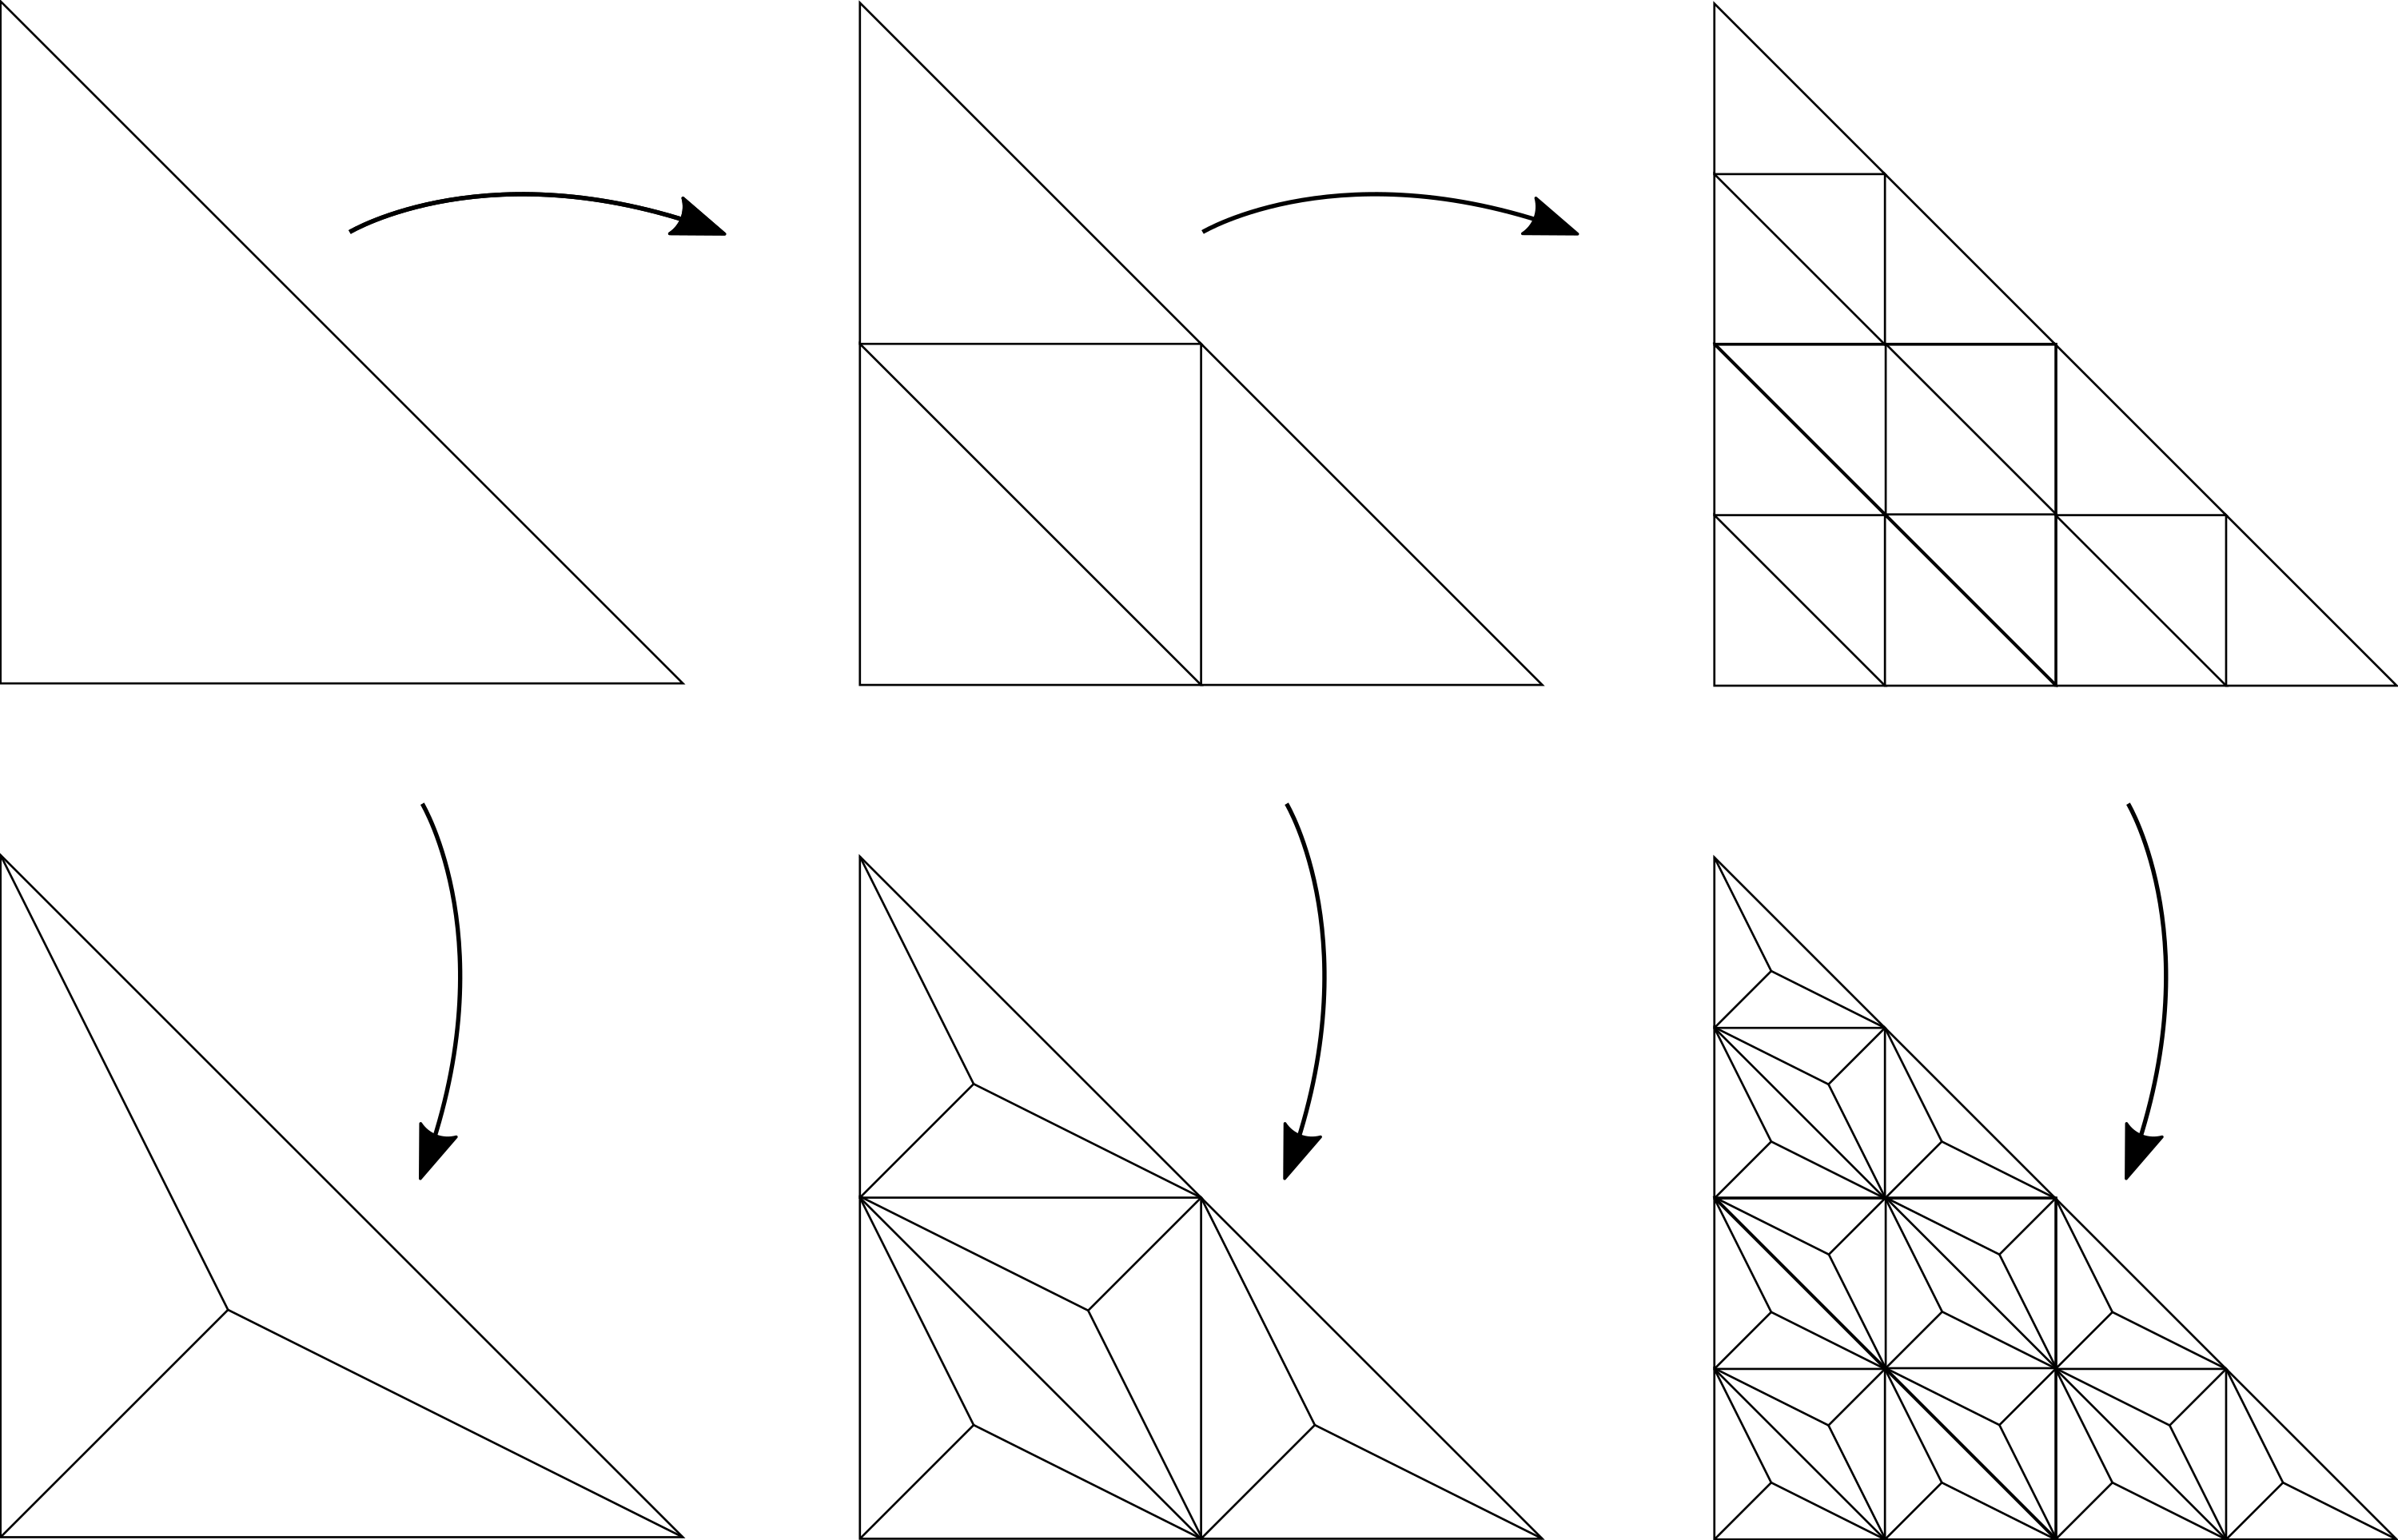
\includegraphics[height=0.4\textheight]{mh_bary_5}
      \end{center}
    \end{onlyenv}
    \begin{onlyenv}<2->
  \begin{columns}
    \begin{column}{0.6\textwidth}
\begin{minted}[fontsize=\scriptsize]{python}
-ksp_type fgmres
-pc_type mg
-mg_levels_
   -ksp_type gmres
   -pc_type python
   -pc_python_type firedrake.PatchPC
   -patch_
      -pc_patch_construct_type python
      -pc_patch_construct_python_type MacroStar
\end{minted}
    \end{column}
    \begin{column}{0.4\textwidth}
      \vspace{-1.5em}
      \begin{center}
        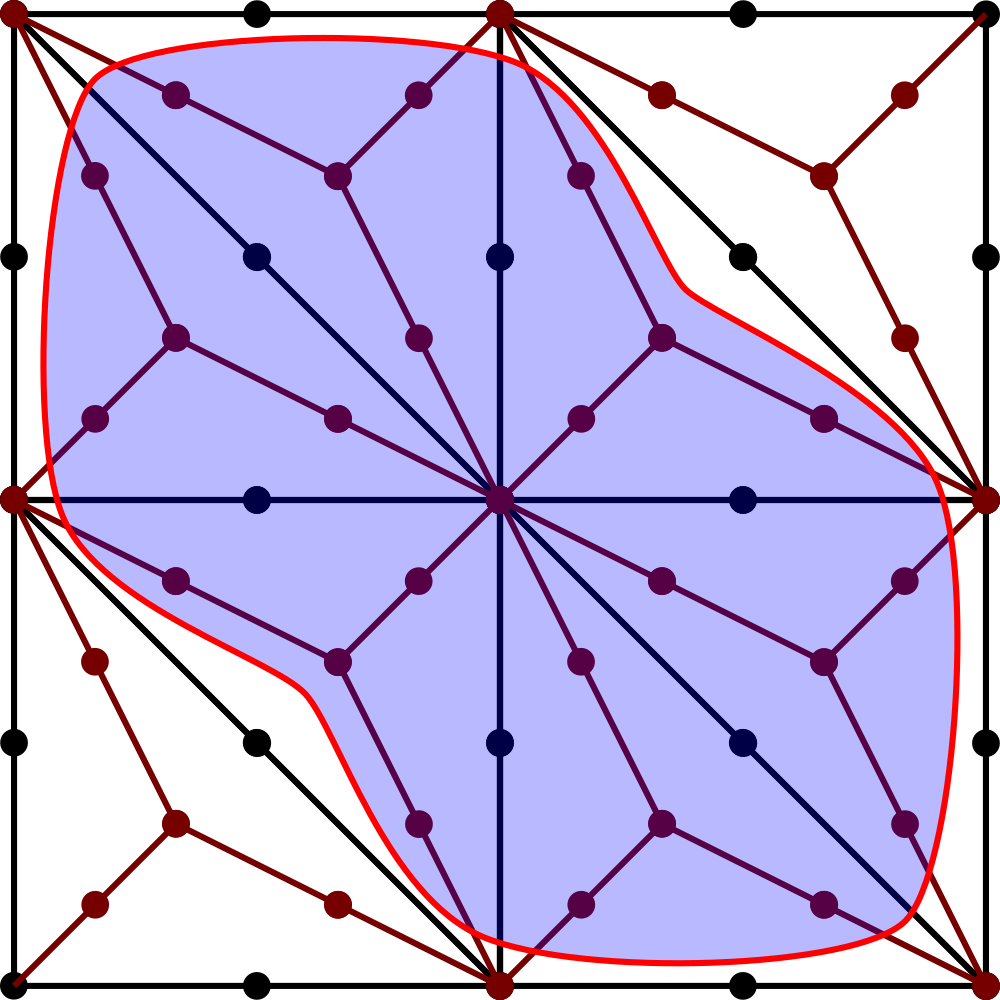
\includegraphics[width=\textwidth]{macrostar}
      \end{center}
    \end{column}
  \end{columns}
    \end{onlyenv}
  \end{overlayarea}
\end{frame}
\begin{frame}
  \frametitle{3D lid-driven cavity}
  \begin{table}[htbp]
    \centering
    \begin{tabular}{cc|ccccc}
      \toprule
      \# ref. & \# dofs & \multicolumn{5}{c}{Reynolds number} \\
              && 10 & 100 & 1\,000 & 2\,500 & 5\,000 \\
      \midrule
      1   & $1.03\times 10^6$     & 3.00  & 3.67  & 3.50 & 4.00 & 5.00\\
      2   & $8.22\times 10^6$     & 3.50  & 3.67  & 4.00 & 4.00 & 4.00\\
      3   & $6.55\times 10^7$     & 3.00  & 3.33  & 3.50 & 3.50 & 4.00\\
      \bottomrule
    \end{tabular}
    \caption{Average number of outer Krylov iterations per Newton step for a
      3D regularised lid-driven cavity problem with
      $(\mathbb{CG}_3)^{2}-\mathbb{DG}_2$ pair.}
  \end{table}
  
  {\raggedleft \scriptsize
    \textcite{Farrell:2021a}
    \arxivlink{2004.09398}{math.NA}\par}
\end{frame}

\begin{frame}
  \frametitle{AL for implicit timestepping}

  \begin{block}{Shallow water with compatible FEM}
    \begin{align*}
      u^{n+1} - u^{n} + \Delta t (u^{n+1/2} \cdot \nabla) u^{n+1/2} +
      \Delta t g h^{n+1/2} \\
      \alert{-\gamma \nabla\left(h^{n+1} - h^n + \Delta t \nabla
      \cdot (h^{n+1/2} u^{n+1/2})\right)} &= 0\\
      h^{n+1} - h^n + \Delta t \nabla \cdot (h^{n+1/2} u^{n+1/2}) &= 0
    \end{align*}
    After discretisation and linearisation, Schur complement
    approximation

    \begin{equation*}
      \tilde{S} \approx \gamma^{-1} L^{-1}(I - g \Delta t/2 L),
    \end{equation*}
    $L$ the Laplacian (or just ignore as $\Delta t \to \infty$).
  \end{block}
\end{frame}
\begin{frame}
  \frametitle{Preliminary results}
  {\scriptsize
    \centering
    \begin{tikzpicture}[%
      every node/.style={draw=black, thick, anchor=west},
      grow via three points={one child at (0.0,-0.7) and
        two children at (0.0,-0.7) and (0.0,-1.4)},
      edge from parent path={(\tikzparentnode.210) |- (\tikzchildnode.west)}]
      \node {Newton solver with line search}
      child { node {Krylov solver (FGMRES)}
        child { node {Block preconditioner}
          child { node {Approximate Schur complement inverse}
            child { node {$\tilde{S}^{-1} = M_\text{DG}^{-1}$ } }
          }
          child [missing] {}
          child { node {Geometric MG}
            child { node {Coarse grid solver}
              child { node {LU factorisation}}
            }
            child [missing] {}
            child { node {Relaxation}
              child { node {GMRES (3 iterations)}
                child { node {ASM smoother}}
              }
            }
          }
        }
      };
    \end{tikzpicture}
    \par}
\end{frame}
\begin{frame}
  \frametitle{Williamson mountain testcase}
  \begin{table}[htbp]
    \centering
    \begin{tabular}{cc|ccccc}
      \toprule
      \# ref. & \# cells & \# $h$ dofs & \# $u$ dofs & FGMRES its\\
      \midrule
      3   & 1280 & 3840 & 9600 & 6--7\\
      4 & 5120  & 15360 & 38400 & 6--7\\
      5 & 20480 & 61440 & 153600 & 6--7\\
      6 & 81920 & 245760 & 614400 & 6--7\\
      7 & 327680 & 983040 & 2457600 & 6--7\\
      \bottomrule
    \end{tabular}
    \caption{Krylov iterations per Newton step with
      $\Delta t = 1\text{hour}$}
  \end{table}

  {\centering
    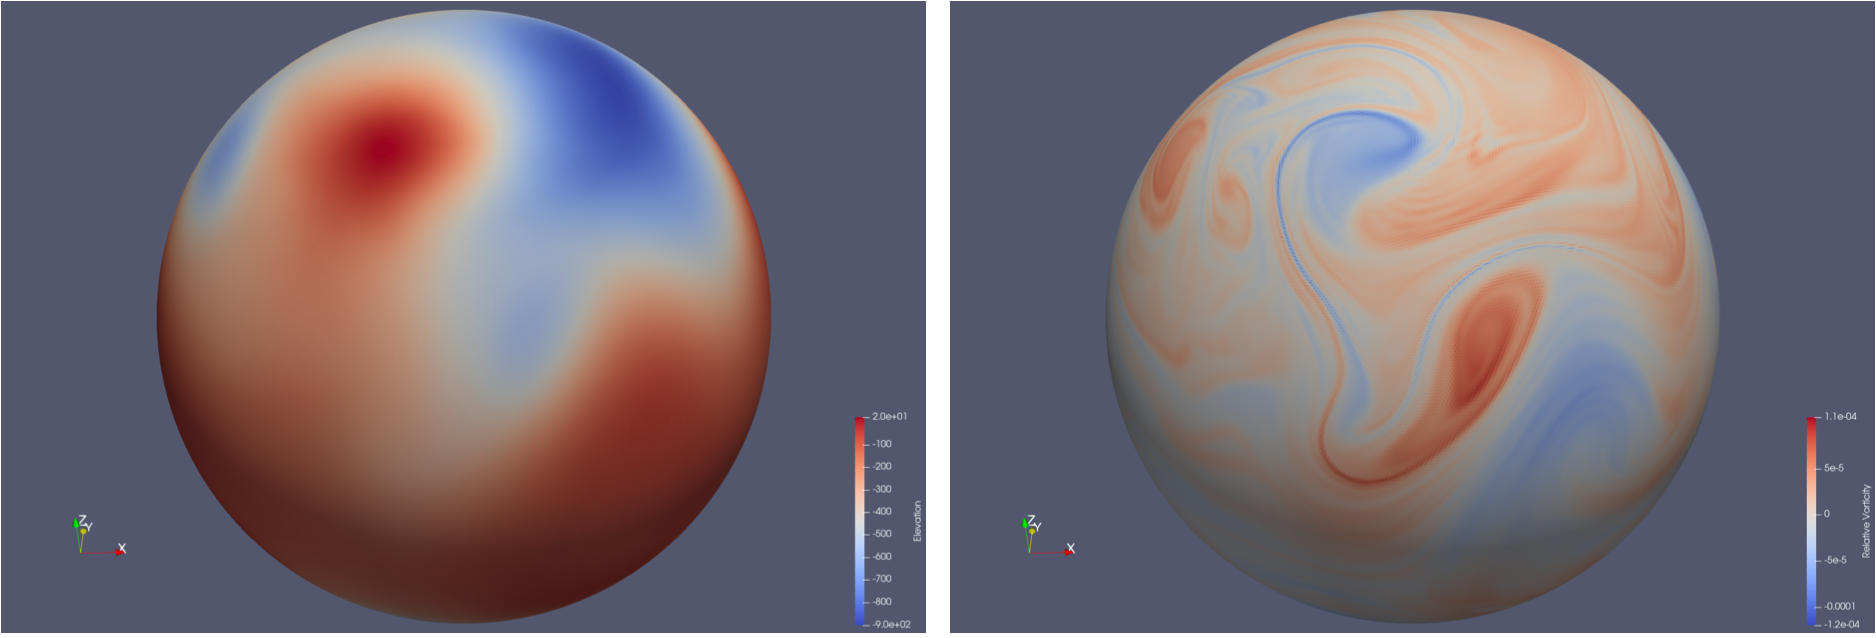
\includegraphics[height=0.4\textheight]{williamson-mountain-al}\par
    }
\end{frame}

\begin{frame}
  \frametitle{Conclusions}
  \begin{itemize}
  \item Bidirectional solver/discretisation interface useful
  \item Playground for preconditioner design: it's easy to get all the
    operators you need
  \item With scalability to large problems
  \item Overlapping Schwarz methods also benefit from this
  \item With topological decompositions in hand, can provide a
    \emph{generic} interface, encompassing many useful smoothing
    schemes
  \item Get stuck on harder problems faster
  \end{itemize}

  \begin{center}
    Thanks!
  \end{center}
\end{frame}

\appendix
\begin{frame}[allowframebreaks]
  \frametitle{References}
  \printbibliography[heading=none]
\end{frame}

\end{document}
% Motivation:
% - Block preconditioning, what to do on blocks, how to deliver
%   auxiliary operators? Or what if the preconditioner is not just the
%   inverse of a single operator?
% - Multigrid with "fancy" smoothers: motivation augmented Lagrangian
%   methods for problems with constraints
%
%   Examples:
%   - Stokes: "Easy"
%   - Stokes: BFBT?; N-S: PCD
%   - Stationary problems: N-S (schur complement + AL)
%   - MHD (probably too much)
%   - Implicit timestepping (Colin's stuff for shallow-water)
%
% - Software
% - PETSc composition philosophy
% - callbacks to discretisation library for all the operators.
% - PCPatch (for the smoothers)

% Things that don't work
% DD (like ffddm)
% PCPatch doesn't work for high order (designed around doing dense
% inverse on assembly patch operators).
% Batching/small solvers
% Interface is necessarily (?) not the same as the full Jacobian
% construction. Design guided by performance?

